\subsection{Arrival time simulation}
\label{sec:arrival_simulation}

To assess the performance of our method, we first prepared a simulation which uses known travel time states for upcoming road segments. From this, we are able to present each component of the predictive model individually.


\begin{knitrout}\small
\definecolor{shadecolor}{rgb}{0.969, 0.969, 0.969}\color{fgcolor}\begin{figure}

{\centering \subfloat[First few stops\label{fig:arrival_simulation1}]{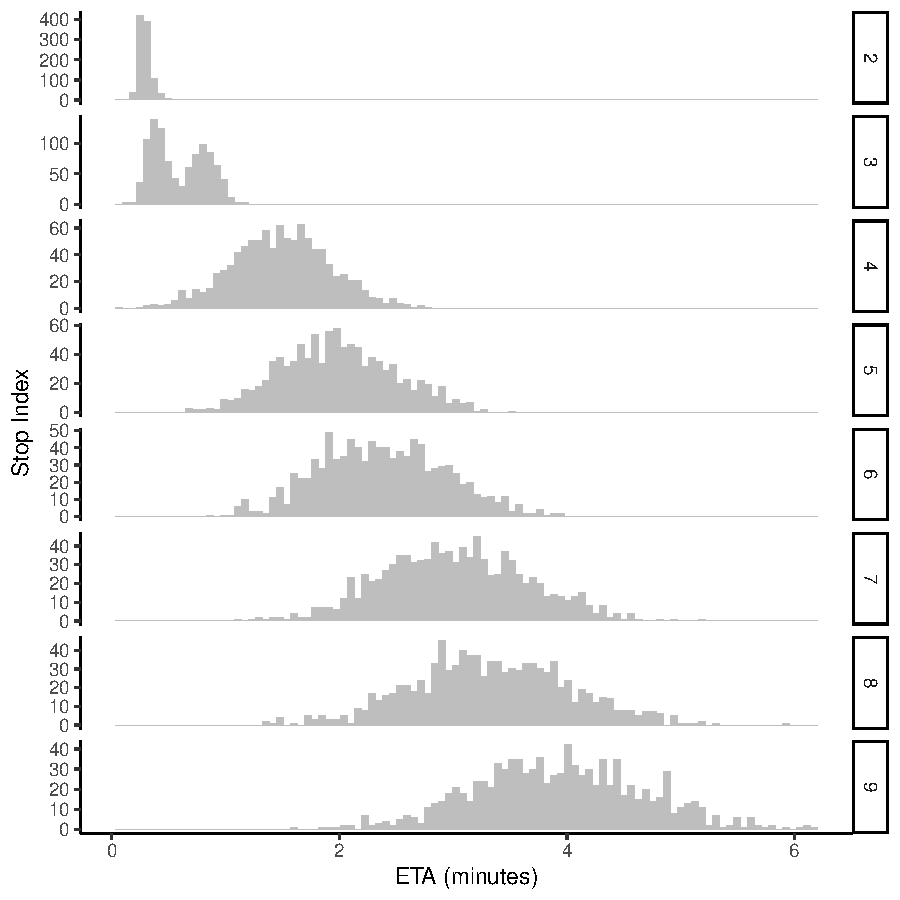
\includegraphics[width=.8\textwidth]{figure/arrival_simulation-1} }\\
\subfloat[Last few stops\label{fig:arrival_simulation2}]{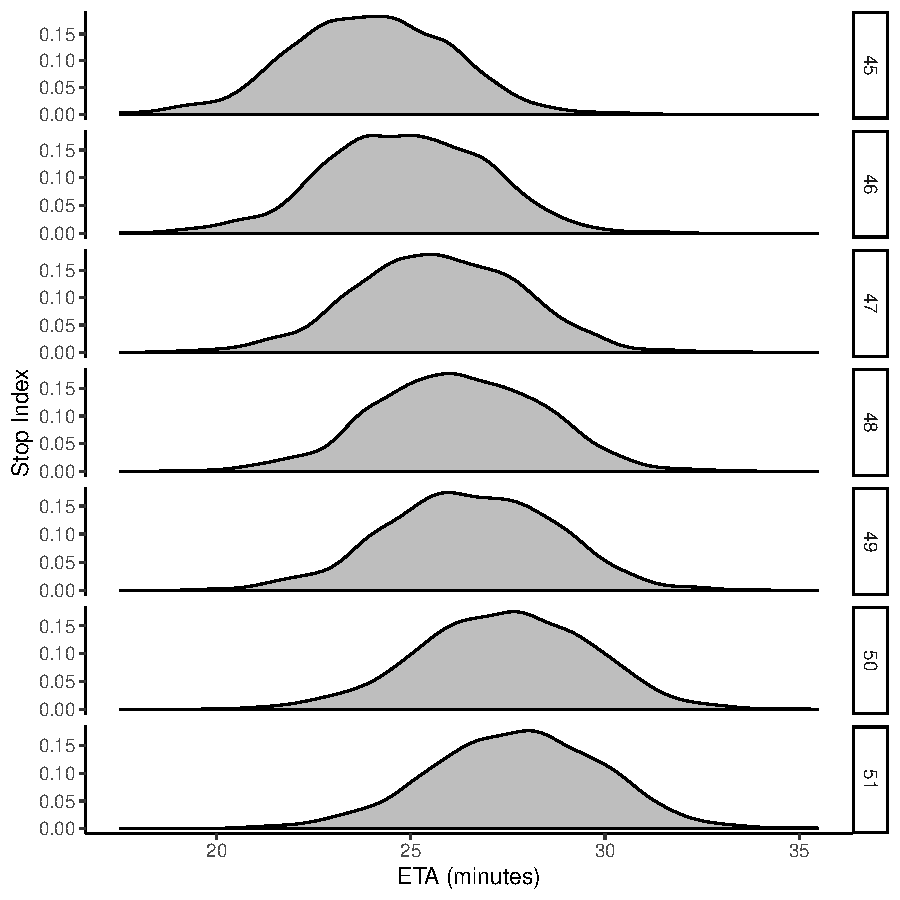
\includegraphics[width=.8\textwidth]{figure/arrival_simulation-2} }\\

}

\caption[ETAs from simulation]{ETAs from simulation.}\label{fig:arrival_simulation}
\end{figure}


\end{knitrout}
